\section{Jacobi  functions: basic properties}
\label{app:appD-jacobi-functions}

Here we review Jacobi's functions and derive some basic properties. For more on this subject see \cite{armitage-2006}.

Let $0<k<1$ and consider the elliptic integral
\[u=F(\varphi,k)=\int_{0}^{\varphi} \frac {dx}{\sqrt {1-k^2   \sin^2 x  
}} \]
The inverse of $F$ will be denoted by $\varphi=\text{am}(u,k)=\text{am}(u)$ and is called the amplitude Jacobi function.

The functions
\begin{align*}
    %
 \cn(u,k)&=\Jcn(u,k)=\cos(\am(u,k))\\ \;
 \sn(u,k)&=\Jsn(u,k)=\sin(\am(u,k))\\
 \dn(u,k)&=\sqrt{1-k^2\sn^2(u,k)}
 \end{align*}
\noindent  are called the Jacobi's elliptic  functions. 
For $k$ fixed they will denoted simply by $\cn(u)$ and $\sn(u).$


\noindent Note: In the software Mathematica these functions are implemented taking $k^2$ as $k$.


From definition basic properties are:

\begin{align*}
\cn(0)&=1,\; \sn(0)=0, \; \dn(0)=1;\\
\cn(K)&=0,\; \sn(K)=1, \; \dn(K)=\sqrt{1-k^2}=k_1\\
\cn(2K)&=-1,\; \sn(2K)=0, \; \dn(2K)=1.
   %
\end{align*}
Also,
\begin{align*}
 \sn^2(u)  &+\cn^2(u) =1\\
 \dn^2 (u)&+k^2\sn^2(u)  =1\\
\sn'(u)&=\cn(u)\dn(u)\\
\cn'(u)&=-\sn(u)\dn(u)\\
\dn'(u)&=-k^2\sn(u)\cn(u)\\
\text{am}'(u)&=\dn(u)
\end{align*}

\begin{align*}
    \cn(u+v)&=\frac{\cn(u)\cn(v)-\sn(u)\sn(v)\dn(u)\dn(v)}{\Delta(u,v)}\\
    \sn(u+v)&=\frac{\sn(u)\cn(v)\dn(v)+\sn(v)\cn(u)\dn(u) }{\Delta(u,v)}\\
    \dn(u+v)&=\frac{\dn(u)\dn(v)-k^2\sn(u)\sn(v)\cn(u)\cn(v) }{\Delta(u,v)}\\
    %
    \Delta(u,v)&=1-k^2\sn^2(u)\,\sn^2(v)
\end{align*}

\begin{figure}[H]
    \begin{center}
    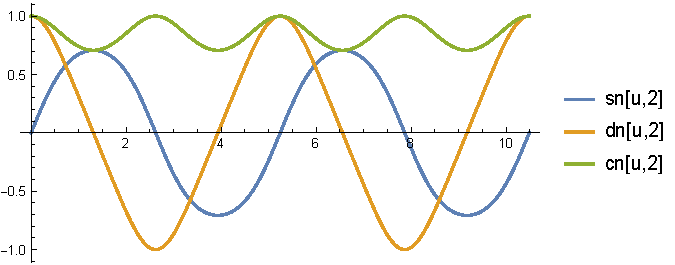
\includegraphics[scale=0.8]{zappD/pics/pics_appD_020_plot_jacobi.pdf}
    \caption{Jacobi elliptic functions}
    \label{fig:jacobi_SCD}
    \end{center}
\end{figure}

We have that $\sn(u,k)$ is solution of the implicit differential equation
\[\left(\frac{dy}{du}\right)^2=(1-y^2)(1-k^2y^2)\]

The function $\cn(u,k)$ is solution of 
\[\left(\frac{dy}{du}\right)^2=(1-y^2)(1-k^2+k^2y^2)\]
and $\dn(u,k)$ is solution of
\[\left(\frac{dy}{du}\right)^2=( y^2-1)(1-k^2-y^2)\]

The inverse of the Jacobi elliptic functions are defined by:
\begin{align*}
  \mathrm{arcsn}(u,k)&=\int_0^u\frac{dy}{\sqrt{(1-y^2)(1-k^2y^2)}}\\
    \mathrm{arccn}(u,k)&=\int_u^1\frac{dy}{\sqrt{(1-y^2)(1-k^2+k^2y^2)}}\\
      \mathrm{arcdn}(u,k)&=\int_u^1\frac{dy}{\sqrt{(1-y^2)( k^2-1+y^2)}}
\end{align*}

Below we recall some   facts about three of Jacobi's elliptic functions extended to the complex plane $sn(z,k)=\sin{(\am(z,k))}$, $cn(z,k)=\cos(\am(z,k))$ and $dn(z,k)=\sqrt{1-k^2sn^2(z,k)}$, where $z \in \mathbb{C}$, and $0<k<1$ is the elliptic modulus. 
%Since $k$ is fixed, we write $sn(z)$ instead of $sn(z,k)$, etc.

These functions have two independent periods and also have simple poles at the same points. In fact:

\begin{align*}
    \sn(u+4K)&=\sn(u+2iK')=\sn(u)\\
    \cn(u+4K)&=\cn(u+2K+2iK')=\cn(u)\\
    \dn(u+2K)&=\dn(u+4iK')=\dn(u)\\
    K'&=K(k'), \;\;k'=\sqrt{1-k^2}
\end{align*}
The  poles of these three functions, which are simple, occur at the points
\[2mK+i(2n+1)K'
,\;\; m,n\in \mathbb{Z}\]

They also display a certain symmetry around the poles. Namely, if $z_p$ is a pole of $\sn(z)$, $\cn(z)$ and $\dn(z)$, then, for every $w \in \mathbb{C}$, we have \cite[Chapter 2]{armitage-2006}:

\begin{align}
\sn(z_p+w)=&-\sn(z_p-w) \nonumber \\
\cn(z_p+w)=&-\cn(z_p-w)  \label{eqn:zpole} \\
\dn(z_p+w)=&-\dn(z_p-w) \nonumber
\end{align}
